\documentclass[acmlarge]{acmart}

\acmConference{Scheme and Functional Programming Workshop 2017}{September 03, 2017}{Oxford, UK}
\acmSubmissionID{}
\acmDOI{}
\setcopyright{none}
\copyrightyear{2017}
\settopmatter{printacmref=false, printccs=false, printfolios=false}
\acmVolume{}
\acmNumber{}
\acmArticle{3}
\acmYear{2017}
\acmMonth{9}
\renewcommand\footnotetextcopyrightpermission[1]{}
\usepackage{fancyhdr}
\pagestyle{fancy}
\fancyfoot{}
\fancyfoot[R]{}
\fancypagestyle{firstfancy}{
\fancyhead{}
\fancyhead[R]{Paper\quad\textbullet\quad3}
\fancyfoot{}
}

\citestyle{acmauthoryear}

\usepackage{mdframed}
\usepackage{booktabs}
\usepackage{enumitem}
\usepackage{amsmath}
\usepackage{amsthm}
\usepackage{color}
\usepackage{calc}
\usepackage{xspace}
\usepackage{upgreek}
\usepackage{graphicx}
\usepackage{natbib}
\usepackage{alltt}
\usepackage{fancyvrb}
\usepackage{array}
\usepackage{tabu}
\usepackage{multirow}
\usepackage{mathpartir}
\usepackage{balance}
\usepackage{subcaption}
\usepackage{wrapfig}
\usepackage{framed}
\usepackage{colortbl}
\usepackage{kbordermatrix}


%\usepackage{courier}
\usepackage[ocr-a]{ocr} % Or whatever TT font we like
%\usepackage[T1]{fontenc}
%%% Hack to suppress a warning
%% \renewcommand*\copyright{{%
%%   \usefont{EU1}{lmr}{m}{n}\textcopyright}}

 
\usepackage{microtype}%if unwanted, comment out or use option "draft"

\definecolor{comment}{rgb}{0.59, 0.72, 0.83}
\definecolor{contract}{rgb}{0.86, 0.64, 0.26}
\definecolor{errstring}{rgb}{0.73, 0.42, 0.34}


%% \acmJournal{}
%% \acmVolume{9}
%% \acmNumber{4}
%% \acmArticle{39}
%% \acmYear{2010}
%% \acmMonth{3}
%% \acmArticleSeq{11}

%\acmBadgeR[http://ctuning.org/ae/ppopp2016.html]{ae-logo}
%\acmBadgeL[http://ctuning.org/ae/ppopp2016.html]{ae-logo}


% Copyright
%\setcopyright{acmcopyright}
%\setcopyright{acmlicensed}
\setcopyright{none}
%\setcopyright{usgov}
%\setcopyright{usgovmixed}
%\setcopyright{cagov}
%\setcopyright{cagovmixed}

% DOI
\acmDOI{0000001.0000001}

% Paper history
%% \received{February 2007}
%% \received{March 2009}
%% \received[accepted]{June 2009}



\begin{document}
\title[Paper: Toward Parallel CFA with Datalog, MPI, and CUDA]{Toward Parallel CFA with Datalog, MPI, and CUDA}

\author{Thomas Gilray}
\affiliation{%
  \institution{University of Maryland}
  \city{College Park}
  \state{MD}
  \country{USA}
}
\author{Sidharth Kumar}
\affiliation{%
  \institution{University of Utah}
  \city{Salt Lake city}
  \state{UT}
  \country{USA}
}


\newcommand{\phrame}{\phi}
\newcommand{\aphrame}{\hat{\phi}}

\newcommand{\defas}{\triangleq}


\newcommand{\var}[1]{\mathit{#1}}
\newcommand{\syn}[1]{\mathsf{#1}}


\newcommand{\Pow}[1]{\mathcal{P}(#1)}
\newcommand{\Set}[1]{\{#1\}}
\newcommand{\SetBuild}[2]{\{#1\ \vert\ #2\}}

\newcommand{\ttlp}{\texttt{(}}
\newcommand{\ttrp}{\texttt{)}}
\newcommand{\sexpr}[1]{\ttlp#1\ttrp}


\newcommand{\join}{\sqcup}
\newcommand{\sqless}{\sqsubseteq}


\newcommand{\parto}{\rightharpoonup}
\newcommand{\aexp}{\var{ae}}


\newcommand{\letform}[3]{\texttt{(let\ ([}#1\ #2\texttt{])\ }#3\texttt{)}}
\newcommand{\appform}[2]{\texttt{(}#1\ #2\texttt{)}}
\newcommand{\lamform}[2]{\texttt{($\lambda$\ (}#1\texttt{)\ }#2\texttt{)}}


\newcommand{\calcTo}{\rightarrow_{\text{calc}}}
\newcommand{\abscalcTo}{\rightarrow_{\text{sign}}}

\newcommand{\lamTo}{\rightarrow_{\scalebox{0.60}{$\lambda$}}}
\newcommand{\cekTo}{\rightarrow_{\scalebox{0.50}{CEK}}}

\newcommand{\instTo}{\overset{\scalebox{0.40}{\!\!\!\!Inst}}{\leadsto}}
\newcommand{\instToEmpty}{\leadsto^{0}_{\scalebox{0.50}{Inst}}}


\newcommand{\cTo}{\rightarrow_{\scalebox{0.45}{$\Sigma$}}}
\newcommand{\cToW}{\rightarrow_{\scalebox{0.45}{$S$}}}
\newcommand{\fsTo}{\leadsto^{\text{\texttildelow}}_{\scalebox{0.45}{$\Sigma$}}}
\newcommand{\pdTo}{\leadsto^{\scalebox{0.45}[0.25]{$\wedge$}}_{\scalebox{0.45}{$\Sigma$}}}
\newcommand{\fsToW}{\leadsto^{\text{\texttildelow}}_{\scalebox{0.45}{$\Xi$}}}
\newcommand{\pdToW}{\leadsto^{\scalebox{0.45}[0.25]{$\wedge$}}_{\scalebox{0.45}{$\Xi$}}}
\newcommand{\fsToS}{\leadsto^{\text{\texttildelow}}_{\scalebox{0.45}{$S$}}}
\newcommand{\pdToS}{\leadsto^{\scalebox{0.45}[0.25]{$\wedge$}}_{\scalebox{0.45}{$S$}}}
\newcommand{\pdToX}{\leadsto^{\scalebox{0.45}[0.25]{$\wedge$}}_{\scalebox{0.45}{$\mathcal{X}$}}}
\newcommand{\dsToW}{\leadsto^{\scalebox{0.45}[0.25]{$\wedge$}}_{\scalebox{0.45}{$G$}}}
\newcommand{\pdToSub}{\overset{\scalebox{0.45}[0.45]{$\!\!\!\!\!\sqsubseteq$}}{\leadsto^{\scalebox{0.45}[0.25]{$\wedge$}}_{\scalebox{0.45}{$\Sigma$}}}}
\newcommand{\fsToSub}{\overset{\scalebox{0.45}[0.45]{$\!\!\!\!\!\sqsubseteq$}}{\leadsto^{\text{\texttildelow}}_{\scalebox{0.45}{$\Sigma$}}}}
\newcommand{\fsPath}{\overset{\!\scalebox{0.55}[0.55]{\texttildelow}}{\hookrightarrow}}
\newcommand{\pdPath}{\overset{\!\scalebox{0.45}[0.25]{$\wedge$}}{\hookrightarrow}}



\newcommand{\simXi}{\sqsupseteq_{\scalebox{0.5}{$\Xi$}}}
\newcommand{\simState}{\sqsupseteq_{\scalebox{0.45}{$\Sigma$}}}
\newcommand{\simR}{\sqsupseteq_{\scalebox{0.45}{$R$}}}
\newcommand{\simX}{\sqsupseteq_{\scalebox{0.45}{$\mathcal{X}$}}}
\newcommand{\simEnv}{\equiv_{\scalebox{0.45}{$Env$}}}
\newcommand{\simAddr}{\equiv_{\scalebox{0.45}{$Addr$}}}
\newcommand{\simStore}{\sqsupseteq_{\scalebox{0.45}{$Store$}}}
\newcommand{\simD}{\sqsupseteq_{\scalebox{0.45}{$D$}}}
\newcommand{\simClo}{\equiv_{\scalebox{0.45}{$Clo$}}}
\newcommand{\simKont}{\sqsupseteq_{\scalebox{0.45}{$Kont$}}}
\newcommand{\simFrame}{\equiv_{\scalebox{0.45}{$Frame$}}}
\newcommand{\simTau}{\equiv_{\scalebox{0.45}{$\tau$}}}

\newcommand{\precXi}{\sqsupseteq_{\scalebox{0.5}{$\Xi$}}}
\newcommand{\precStore}{\sqsupseteq_{\scalebox{0.45}{$Store$}}}
\newcommand{\precD}{\sqsupseteq_{\scalebox{0.45}{$D$}}}
\newcommand{\precR}{\sqsupseteq_{\scalebox{0.45}{$R$}}}

\newcommand{\tAddr}{T_{\scalebox{0.45}[0.45]{$Addr$}}}
\newcommand{\tEnv}{T_{\scalebox{0.45}[0.45]{$Env$}}}
\newcommand{\tClo}{T_{\scalebox{0.45}[0.45]{$Clo$}}}
\newcommand{\tD}{T_{\scalebox{0.45}[0.45]{$D$}}}
\newcommand{\tStore}{T_{\scalebox{0.45}[0.45]{$Store$}}}
\newcommand{\tFrame}{T_{\scalebox{0.45}[0.45]{$Frame$}}}
\newcommand{\tTau}{T_{\scalebox{0.65}[0.65]{$\tau$}}}

\newcommand{\hAddr}{H_{\scalebox{0.45}[0.45]{$Addr$}}}
\newcommand{\hEnv}{H_{\scalebox{0.45}[0.45]{$Env$}}}
\newcommand{\hClo}{H_{\scalebox{0.45}[0.45]{$Clo$}}}
\newcommand{\hD}{H_{\scalebox{0.45}[0.45]{$D$}}}
\newcommand{\hStore}{H_{\scalebox{0.45}[0.45]{$Store$}}}
\newcommand{\hFrame}{H_{\scalebox{0.45}[0.45]{$Frame$}}}
\newcommand{\hKont}{H_{\scalebox{0.45}[0.45]{$Kont$}}}
\newcommand{\hC}{H_{\scalebox{0.45}[0.45]{$C$}}}
\newcommand{\hState}{H_{\scalebox{0.45}[0.45]{$\Sigma$}}}
\newcommand{\hTau}{H_{\scalebox{0.65}[0.65]{$\tau$}}}

\newcommand{\inpsi}{\in_{\scalebox{0.7}[0.7]{$\psi$}}}



\newcommand{\simGenericprec}{\overset{\scalebox{0.45}{$\!\!\!\sqsupseteq$}}{\equiv}}

%\techreporttrue

\begin{abstract} 
%
  We present our recent experience working to design parallel functional control-flow analysis (CFA)
  using an encoding in Datalog and underlying relational algebra implemented for SIMD coprocessors and supercomputers.
  %
  Control-flow analysis statically models the possible propagations of data and control through
  a target program, finitely obtaining a bound on reachable expressions and environments and on 
  possible return and argument values.
  %
  We used Souffl\'e, a parallel CPU-based Datalog implementation from Oracle labs, and
  worked toward a new MPI-based distributed hash join implementation and an extension of the
  GPU-based relational algebra library RedFox.

  
  In this paper, we provide introductions to functional flow analysis, Datalog, MPI, and CUDA, explaining the total
  process we are working on to bring these components together in an analysis pipeline toward the end of scaling
  functional program analyses by extracting their intrinsic parallelism in a principled manner.
%
\end{abstract}

\keywords{Control-flow analysis; CFA; Datalog; CUDA; MPI; Parallelism; Static analysis}

\maketitle 
\thispagestyle{firstfancy}


\section{Introduction}
%
A \textit{control-flow analysis} (CFA) of a functional programming language models the
propagation of data flows and control flows through a target program, across all
possible executions.
%
In static analyses of functional languages generally, a model of where functional values
(i.e., lambdas, closures) can flow is required to model where control can flow
from a call site, and vice versa.
%
At a call site in Scheme, \texttt{(f x)}, the possible values for \texttt{f} determine
which lambda bodies can be reached.
%
Likewise, the possible callers for the lambda that binds \texttt{f},
$\texttt{(lambda ($\ldots$ f $\ldots$) $\ldots$)}$, influence the lambdas that
can flow into \texttt{f}.
%
This mutual dependence of data flow and control flow can be handled using an abstract interpretation,
simultaneously modeling all interdependent language features.
%
There are systematic approaches to designing analyses such as these, however the traditional worklist algorithms
used to implement them in practice are inefficient and have difficulty scaling.
%
Even with optimizations such as global-store widening and flat environments, the analysis is in $O(n^3)$ in the
flow-insensitive case or in $O(n^4)$ in the flow-sensitive case.
%
Using more advanced forms of polyvariance or context-sensitivity, the analysis becomes significantly more expensive.


In this paper, we describe our ongoing work to encode these analyses as declarative datalog programs and
implement them as highly parallel relational algebra (RA), on the GPU and across many CPUs.
%
Relational algebra operations, derived from Datalog analysis specifications, are computationally intensive and memory-bound in nature.
%
GPUs provide massive fine-grained parallelism and great memory bandwidth, potentially making them the ideal
target for solving these operations. We use Redfox~\cite{Wu:2014:RFE:2581122.2544166}, an open source tool which 
executes queries expressed in a specialized query language on GPUs. We also modify Redfox, adding
capabilities to perform fixed-point iterations essential for solving RA operations derived from Datalog.
%
We are also pursuing a Message Passing Interface (MPI)-based backend for solving RA operations across many compute nodes on a network. 
This approach is also particularly promising, given that HPC is increasingly mainstream and supercomputers are getting
faster cores and lower latency interconnects.






\section{Control-flow Analysis} 
\label{sec:aam}
%
This section introduces control-flow analysis by instantiating it for the continuation-passing-style (CPS)
$\lambda$-calculus. 
%
We follow the abstracting abstract machines (AAM) methodology, a systematic process for developing a static analysis
(an approximating semantics) from a precise operational semantics of an abstract machine.


Static analysis by abstract interpretation proves properties of a program by running code through an interpreter powered by an 
\textit{abstract semantics} that approximates the behavior of an exact \textit{concrete semantics}.
%
This process is a general method for analyzing programs and serves applications such as program verification, malware/vulnerability detection, and
compiler optimization, among others 
\cite{cousot:1976:staticdetermination,cousot:1977:unifiedlatticemodel,cousot:1979:systematicdesign,midtgaard:2012:cfa}.
%
Van Horn and Might's approach of \textit{abstracting abstract machines} (AAM) uses abstract interpretation of abstract machines for \textit{control-flow analysis} (CFA) of functional (higher-order) 
programming languages \cite{johnson:2013:oaam,might:2010:aam,might:2010:free}.
%
The AAM methodology is flexible and allows a high degree of control over how program states are represented.
%
AAM provides a general method for automatically abstracting an arbitrary small-step 
abstract-machine semantics to obtain an approximation in a variety of styles.
%
Importantly, one such style aims to focus all unboundedness in a semantics on the machine's address-space.
%
This makes the strategy used for the allocation of addresses crucial to the tradeoff struck between precision and complexity~\cite{gilray:2016:allocation}, and results in a highly flexible and tunable analysis infrastructure.
%
More broadly, the approach has been used to instantiate both traditional finite flow analyses and heavy-weight program verification \cite{nguyen:2014:SCV}. 


\subsection{A Concrete Operational Semantics}
\label{sec:aam:concrete}
%
This section reviews the process of producing a formal operational semantics for a simple language \cite{plotkin:1981:structural},
specifically, the untyped $\lambda$-calculus in \textit{continuation-passing style} (CPS).
%
CPS constrains call sites to tail position so that functions may never return; instead, callers explicitly pass a continuation forward to be invoked on the return value \cite{plotkin:1975:cps}.
%
This makes our semantics tail recursive (small-step) and easier to abstract while entirely eliding the challenges of manually managing a stack and its abstraction, a process previously discussed in the context of AAM \cite{might:2010:aam, johnson:2014:aac}.
%
Using an AAM that explicitly models the stack in a precise manner, while allowing for adjustable allocation, has also been recently addressed \cite{gilray:2016:p4f}.


The grammar structurally distinguishes between call-sites $call$ and atomic-expressions $ae$:
%
\begin{align*}
	\var{call} \in \syn{Call} ::=&\ \ttlp \var{ae}\ \var{ae}\ \ldots \ttrp\ \vert\ \ttlp \mathtt{halt} \ttrp  
  \\
	\var{lam} \in \syn{Lam} ::=&\ \ttlp \lambda\ \ttlp x\ \ldots \ttrp\ \var{call} \ttrp 
  \\
	\var{ae} \in \syn{AE} ::=&\ \var{lam}\ \vert\ x  
  \\
	x \in \syn{Var} \textit{\ is}&\textit{\ a set of program variables}
\end{align*}
%
Instead of specifically affixing each expression with a unique label, we assume two identical expressions occurring separately in a program are not equal.
%
While a direct-style language with a variety of continuations (e.g., argument continuations, \texttt{let}-continuations, etc.), 
or extensions such as recursive-binding forms, conditionals, mutation, or primitive operations, 
would add complexity to any semantics, they do not affect the concepts we are exploring and so are left out.


We define the evaluation of programs in this language using a relation ($\cTo$), over states of an abstract-machine, which determines how the 
machine transitions from one state to another.
%
States $(\varsigma)$ range over control expression (a call site), binding environment, and value store components:
%
\begin{align*}
  \varsigma \in \Sigma \defas&\ \syn{Call} \times \var{Env} \times \var{Store} 
  \\
  \rho \in \var{Env} \defas&\ \syn{Var} \rightharpoonup \var{Addr}  
  \\
  \sigma \in \var{Store} \defas&\ \var{Addr} \rightharpoonup \var{Value}  
  \\
  a \in \var{Addr} \defas&\ \syn{Var} \times \mathbb{N} 
  \\
  v \in \var{Value} \defas&\ \var{Clo}
  \\
  \var{clo} \in \var{Clo} \defas&\ \syn{Lam} \times \var{Env} 
\end{align*}
%
Environments $(\rho)$ map variables in scope to an address for the visible binding.
%
Value stores $(\sigma)$ map these addresses to values (in this case, closures); these may be thought of as a model of the heap.
%
Both these functions are partial and accumulate points as execution progresses.


Evaluation of atomic expressions is handled by an auxiliary function $(\mathcal{A})$ which produces a value $(\var{clo})$
for an atomic expression in the context of a state $(\varsigma)$.
%
This is done by a lookup in the environment and store for variable references $(x)$, and by closure creation for $\lambda$-abstractions $(\var{lam})$.
%
In a language containing syntactic literals, these would be translated into equivalent semantic values here.
%
\begin{align*}
  \mathcal{A} : \mathsf{AE} \times \Sigma \rightharpoonup&\ \var{Value} 
  \\
  \mathcal{A}(x,\ (\var{call},\ \rho,\ \sigma)) \defas&\ \sigma(\rho(x)) 
  \\
  \mathcal{A}(\var{lam},\ (\var{call},\ \rho,\ \sigma)) \defas&\ (\var{lam},\ \rho) 
\end{align*}


The transition relation $(\cTo) : \Sigma \rightharpoonup \Sigma$ yields at most one successor for a given predecessor in the state-space $\Sigma$.
%
This is defined:
%
\begin{align*} 
  \overbrace{(\ttlp \var{ae}_f\ \var{ae}_1\ \ldots\ \var{ae}_j \ttrp, \rho, \sigma)}^{\varsigma} 
  \cTo 
  (\var{call}', \rho', \sigma')
\end{align*}
\vspace{-0.5cm}
\begin{align*}
  \textrm{where} \ \ \ \ \ \ & (\lamform{x_0 \ldots x_j}{\var{call}'}, \rho_\lambda) = \mathcal{A}(\var{ae}_f,\ \varsigma) 
  \\
  & v_i = \mathcal{A}(\var{ae}_i,\ \varsigma)  
  \\
  & \rho' = \rho_\lambda [ x_i \mapsto a_i ]
  \\
  & \sigma' = \sigma [ a_i \mapsto v_i ]
  \\
  & a_i = (x_i, \vert \var{dom}(\sigma) \vert)
\end{align*}
%
Execution steps to the call-site body of the lambda invoked (as given by the atomic-evaluation of $\var{ae}_f$).
%
This closure's environment $(\rho_\lambda)$ is extended with a binding for each variable $x_i$ to a fresh address $a_i$.
%
A particular strategy for allocating a fresh address is to pair the variable being allocated for with the current number of points in the store (a value that increases after each set of new allocations).
%
The store is extended with the atomic evaluation of $\var{ae}_i$ for each of these addresses $a_i$.
%
A state becomes stuck if \texttt{(halt)} is reached or if the program is malformed (\textit{e.g.}, a free variable is encountered).


To fully evaluate a program $\var{call}_0$ using these transition rules, we \textit{inject} it into our state space using a helper 
$\mathcal{I} : \syn{Call} \to \Sigma$:
%
\begin{align*}
  \mathcal{I}(\var{call}) \defas (\var{call}, \varnothing, \varnothing)
\end{align*}


We may now perform the standard lifting of $(\cTo)$ to a collecting semantics defined over sets of states:
%
\begin{align*}
  s \in S \defas \mathcal{P}(\Sigma)
\end{align*}
%
Our collecting relation $(\cToW)$ is a monotonic, total function that gives a set including the trivially reachable state $\mathcal{I}(\var{call}_0)$
plus the set of all states immediately succeeding those in its input.
%
\begin{align*}
  s \cToW \Set{ \varsigma'\ \vert\ \varsigma \in s \wedge \varsigma \cTo \varsigma' } \cup \Set{ \mathcal{I}(\var{call}_0) }
\end{align*}


If the program $\var{call}_0$ terminates, iteration of $(\cToW)$ from $\bot$ (i.e., the empty set $\varnothing$) does as well.
%
That is, ${(\cToW)}^{n}(\bot)$ is a fixed point containing $\var{call}_0$'s full program trace for some $n \in \mathbb{N}$ whenever $\var{call}_0$ is a terminating program.
%
No such $n$ is guaranteed to exist in the general case (when $\var{call}_0$ is a non-terminating program)
as our language (the untyped CPS $\lambda$-calculus) is Turing-equivalent, our semantics is fully precise, and the state-space we defined is infinite.


\subsection{An Abstract Operational Semantics}
\label{sec:aam:abstract}
%
Now that we have formalized program evaluation using our concrete semantics as iteration to a (possibly infinite) fixed point, we are ready to design a 
computable approximation of this fixed point (the exact program trace) using abstract interpretation.
%
Previous work has explored a wide variety of approaches to systematically abstracting a semantics like these 
\cite{might:2010:aam,johnson:2013:oaam,might:2010:free}.
%%%% ^^ more references here ^^
%
Broadly construed, the nature of these changes is to simultaneously finitize the domains of our machine while introducing non-determinism both into the 
transition relation (multiple successor states may immediately follow a predecessor state) and the store (multiple values may become conflated at a single address).
%
We use a finite address space to cut the otherwise mutually recursive structure of values (closures) and environments.
%
(Without addresses and a value store, environments map variables directly to closures and closures contain environments). 
% 
A finite address space yields a finite state space overall and ensures the computability of our analysis.
%
Typographically, components unique to this \textit{abstract} abstract machine wear hats so we can tell them apart without confusing essential underlying roles:
%
\begin{align*}
  \hat{\varsigma} \in \hat{\Sigma} \defas&\ \mathsf{Call} \times \widehat{\var{Env}} \times \widehat{\var{Store}}
  \\
  \hat{\rho} \in \widehat{\var{Env}} \defas&\ \mathsf{\var{Var}} \rightharpoonup \widehat{\var{Addr}}  
  \\
  \hat{\sigma} \in \widehat{\var{Store}} \defas&\ \widehat{\var{Addr}} \rightarrow \widehat{\var{Value}}  
  \\
  \hat{a} \in \widehat{\var{Addr}} \defas&\ \mathsf{Var}
  \\
  \hat{v} \in \widehat{\var{Value}} \defas&\ \mathcal{P}(\widehat{\var{Clo}})  
  \\
  \widehat{\var{clo}} \in \widehat{\var{Clo}} \defas&\ \mathsf{Lam} \times \widehat{\var{Env}} 
\end{align*}
%
Value stores are now total functions mapping abstract addresses to a \textit{flow set} ($\hat{v}$) of zero or more abstract closures. 
%
This allows a range of values to merge and inhabit a single abstract address, introducing imprecision into our abstract semantics, but also allowing
for a finite state space and a guarantee of computability.
%
To begin, we use a monovariant address set $\widehat{\var{Addr}}$ with a single address for each syntactic variable.
%
This choice (and its alternatives) is at the heart of our present topic and will be returned to shortly.



Evaluation of atomic expressions is handled by an auxiliary function $(\hat{\mathcal{A}})$ which produces a flow set $(\hat{v})$
for an atomic expression in the context of an abstract state $(\hat{\varsigma})$.
%
In the case of closure creation, a singleton flow set is produced.
%
\begin{align*}
  \hat{\mathcal{A}} : \mathsf{AE} \times \hat{\Sigma} \rightharpoonup&\ \widehat{\var{Value}} 
  \\
  \hat{\mathcal{A}}(x,\ (\var{call},\ \hat{\rho},\ \hat{\sigma})) \defas&\ \hat{\sigma}(\hat{\rho}(x)) 
  \\
  \hat{\mathcal{A}}(\var{lam},\ (\var{call},\ \hat{\rho},\ \hat{\sigma})) \defas&\ \Set{(\var{lam},\ \hat{\rho})} 
\end{align*}


The abstract transition relation $(\pdTo) \subseteq \hat{\Sigma} \times \hat{\Sigma}$ yields any number of successors for a given predecessor in the state-space $\hat{\Sigma}$.
%
As mentioned when introducing AAM, there are two fundamental changes required using this approach. 
%
Because abstract addresses can become bound to multiple closures in the store and atomic evaluation produces a flow set containing zero or more closures, one successor state
results for each closure bound to the address for $\var{ae}_f$.
%
Also, due to the relationality of abstract stores, we can no longer use strong update when extending the store $\hat{\sigma}'$.
%
\begin{align*} 
  \overbrace{(\sexpr{\var{ae}_f\ \var{ae}_1\ \ldots\ \var{ae}_j}, \hat{\rho}, \hat{\sigma})}^{\hat{\varsigma}} 
  \pdTo 
  (\var{call}', \hat{\rho}', \hat{\sigma}')
\end{align*}
\vspace{-0.5cm}
\begin{align*}
  \textrm{where} \ \ \ \ \ \ & (\lamform{x_0 \ldots x_j}{\var{call}'}, \hat{\rho}_\lambda) \in \hat{\mathcal{A}}(\var{ae}_f,\ \hat{\varsigma}) 
  \\
  & \hat{v}_i = \hat{\mathcal{A}}(\var{ae}_i,\ \hat{\varsigma})  
  \\
  & \hat{\rho}' = \hat{\rho}_\lambda [ x_i \mapsto \hat{a}_i ]
  \\
  & \hat{\sigma}' = \hat{\sigma} \sqcup [ \hat{a}_i \mapsto \hat{v}_i ]
  \\
  & \hat{a}_i = x_i
\end{align*}
%
A weak update is performed on the store instead which results in the least upper bound of the existing store and each new binding.
%
Join on abstract stores distributes point-wise:
%
\begin{align*}
  \hat{\sigma} \sqcup \hat{\sigma}' &\defas \lambda \hat{a}.\ \hat{\sigma}(\hat{a}) \cup \hat{\sigma}'(\hat{a})
\end{align*}
%
Unless it is desirable, and provably safe to do so \cite{might:2006:gammacfa}, we never remove closures already seen.
%
Instead, we strictly accumulate every closure bound to each $\hat{a}$ (i.e., abstract closures which simulate closures bound to addresses which $\hat{a}$ simulates)
over the lifetime of the program.
%
A flow set for an address $\hat{a}$ indicates a range of values which over-approximates all possible concrete values that can flow to any 
concrete address approximated by $\hat{a}$.
%
For example, if a concrete machine binds $(y, 345) \mapsto \var{clo}_1$ and $(y, 903) \mapsto \var{clo}_2$, 
its monovariant approximation might bind $y \mapsto \{ \widehat{\var{clo}}_1, \widehat{\var{clo}}_2 \}$.
%
Precision is lost for $(y, 345)$ both because its value has been merged with $\widehat{clo}_2$, and because the environments for $\widehat{clo}_1$ and 
$\widehat{clo}_2$ in-turn generalize over many possible addresses for their free variables (the environment in $\widehat{\var{clo}}_1$ is less precise than that in $\var{clo}_1$).


To approximately evaluate a program according to these abstract semantics, we first define an abstract injection function,
$\hat{\mathcal{I}}$, where the store begins as a function, $\bot$, that maps every abstract address to the empty set.
%
\begin{align*}
 \hat{\mathcal{I}} :&\ \syn{Call} \to \hat{\Sigma}
 \\
 \hat{\mathcal{I}}(\var{call}) \defas&\ (\var{call}, \varnothing, \bot)
\end{align*}


We again lift $(\pdTo)$ to obtain a collecting semantics $(\pdToS)$ defined over sets of states:
%
\begin{align*}
  \hat{s} \in \hat{S} &\defas \Pow{\hat{\Sigma}}
\end{align*}
%
Our collecting relation $(\pdToS)$ is a monotonic, total function that gives a set including the trivially reachable finite-state $\hat{\mathcal{I}}(\var{call}_0)$
plus the set of all states immediately succeeding those in its input. 
%
\begin{align*}
  \hat{s} \pdToS \hat{s}', \text{where}
\end{align*}
\vspace{-0.6cm}
\begin{align*}
  %\text{where}\ \ \ \ \ \ 
  \hat{s}' = \Set{ \hat{\varsigma}'\ \vert\ \hat{\varsigma} \in \hat{s} \wedge \hat{\varsigma} \pdTo \hat{\varsigma}' } \cup \Set{ \hat{\mathcal{I}}(\var{call}_0) }
\end{align*}
%
Because $\widehat{Addr}$ (and thus $\hat{\Sigma}$) is now finite, we know the approximate evaluation of even a non-terminating $\var{call}_0$ will terminate.
%
That is, for some $n \in \mathbb{N}$, the value $(\pdToS)^{n}(\bot)$ is guaranteed to be a fixed point containing an approximation of $\var{call}_0$'s full concrete program trace
\cite{tarski:1955:fixpoint}.



\subsubsection{Widening and Extension to Larger Languages}
\label{sec:aam:extension}
%
Various forms of widening and further approximations may be layered on top of the na\"ive analysis ($\pdToS$).
%
One such approximation is store widening, which is necessary for our analysis to be polynomial-time in the size of the program.
%
This structurally approximates the analysis above, where each state contains a whole store, by pairing a set of states without stores, with a single, global store that overapproximates all possible bindings.
%
This global store is maintained as the least-upper-bound of all bindings that are encountered in the course of analysis.



Setting up a semantics for real language features such as conditionals, primitive operations, direct-style recursion, 
or exceptions, is no more difficult, if more verbose.
%
Supporting direct-style recursion, for example, requires an explicit stack as continuations are no longer baked into the 
source text by CPS conversion.
%
Handling other forms is often as straightforward as including an additional transition rule for each.
%





\section{Datalog-based Flow Analysis}
%
In this section, we will give an overview of Datalog as a declarative logic-programming
language, show how it may be executed using a bottom-up fixed-point algorithm, and discuss
our encoding of abstract semantics from the previous section.
%



\subsection{Datalog}
%
A datalog program consists of a set of relations, along with the \textit{rules}
pertaining to them.
%
A relation encodes a set of tuples known as \textit{facts}.
%
For example, if we have a relation $\var{Parent}$, the fact $\var{Parent}(p,c)$
may assert that $p$ is a parent of $c$.
%
A rule then takes the form $a_0\ :\!-\ a_1, \ldots, a_j$ where a comma denotes conjunction and
each atom $a_i$ is of the form $r(x, \ldots)$, where $r$ is a relation and each $x$ is a variable.
%
In Datalog the turnstile means ``is implied by''; this is because the rules are formally an implication
form of a Horn clause.
%
Horn clauses are disjunctions where all but one of the atoms are negated: $a_0 \vee \neg a_1 \vee \ldots \vee \neg a_j$.
%
This is the same as $a_0 \vee \neg (a_1 \wedge \ldots \wedge a_j)$ by De Morgan's laws, which is the same as an implication:
$a_0 \impliedby a_1 \wedge \ldots \wedge a_j$.
%
%The satisfiability (SAT) problem for conjunctions of horn clauses (or datalog rules) is complete for PTIME \cite{}. 
%
For example, a rule for computing grandparents can be specified:
%
\[
  \var{GrandParent}(gp, c)\ :\!-\ Parent(gp, p), Parent(p, c).
\]





\subsection{Datalog solvers}
%
A number of strategies exist for executing a datalog program---that is, finding a sound least-fixed-point
that contains all the input facts and obeys every rule.
%
Unlike solvers for Prolog and other logic programming systems, bottom-up approaches have tended to prevail
\cite{ullman:1989:bottomup} although this can depend on extensions to the language and its use.
%
Bottom-up solving begins with the set of facts provided as input, and iterates a monotonic function
encoding the set of rules until a least-fixed-point is reached.
%
The data structure for relations and the operation of these increasing iterations varies by approach.


The datalog solver \textit{bddbddb} uses binary decision diagrams (BDDs) to encode relations and supports
efficient relational algebra (RA) over these structures \cite{whaley:2005:bddbddb}.
%
BDDs are decision trees that encode arbitrary relations by viewing each bit in the input as a binary decision.
%
They have the potential to be a compact and efficient representation of a relation, but have a worst-case
exponential space complexity and are highly sensitive to variable ordering (in what order are bits of input
branched on).


The datalog solver Souffl\'e uses the semi-na\"ive bottom up algorithm with partial-evaluation-based optimization
\cite{scholz:2016:souffle}.
%
A relational algebra machine (RAM) executes the program in bottom-up fashion by using efficient underlying data
structures for relations (such as prefix trees) and directly selects and propagates tuples in a series of nested loops.
%
This RAM then has a partial-evaluation applied to it that optimizes the interpretation for the specific set of
datalog rules.
%
The tool accepts a datalog program as input, performs this partial evaluation and writes a C++ program that
parallelizes the outside loops of each RA operation using pthreads.



\subsection{Encoding CFA}
%
Various program analysis have been implemented using Datalog. Both bddbddb and Souffl\'e presented
program analyses in their experiments. Another prominent example is the DOOP framework for Java
\cite{smaragdakis:2011:pickyourcontexts}, used to demonstrate a generalization of object-sensitive flow analysis.


To encode a control-flow analysis as a Datalog problem, we first represent the abstract syntax tree (AST) as
a set of relations where each expression and variable in the program has been enumerated.
%
In the souffl\'e syntax, the encoding for Lambda expressions, conditional expressions, and Variable references is as follows:
%
\begin{Verbatim}
  .decl SyntaxLambdaExp(e:Exp, x:Var, ebody:Exp) input
  .decl SyntaxIfExp(e:Exp, x:Var, e0:Exp, e1:Exp) input
  .decl SyntaxVarExp(e:Exp, x:Var) input
\end{Verbatim}
%
A tuple $(e_0,x,\var{e_1})$ in the \texttt{SyntaxLambdaExp} relation indicates that the expression $e_0$ is a lambda
with the formal parameter $x$ and the expression body $e_1$. A tuple $(e_0,x,e_1,e_2)$ in the \texttt{SyntaxIfExp} relation
indicates that the expression $e_0$ is a conditional branching on the variable $x$ with the true branch $e_1$ and false
branch $e_2$. A tuple $(e,x)$ in the \texttt{SyntaxVarExp} relation indicates that the expression $e$ is a variable reference
returning the value of variable $x$.


We then encode the constraints of our analysis directly as rules in datalog, such as:
%
\begin{Verbatim}
StoreEdge(x,y) :-
  SyntaxVarExp(e,x),
  ReachableExp(e,kaddr),
  KStore(kaddr,y,ebody,kaddr0).
\end{Verbatim}
%
This rule adds a flow from $x$ to $y$ when a reachable expression $e$ is returning the value at $x$ and
its continuation binds the variable $y$.




\section{Many-node Inner-joins and Future Work}
%
Modern supercomputers' use of very low latency interconnect networks and highly optimized compute cores
opens up the possibility of implementing highly parallel relational algebra using Message-Passing Interface (MPI).
MPI is a portable standard library interface for writing parallel programs in a HPC setting 
and has been highly optimized on a variety of computing infrastructures, from small clusters to high-end supercomputers. 

\begin{figure}
	\centering
	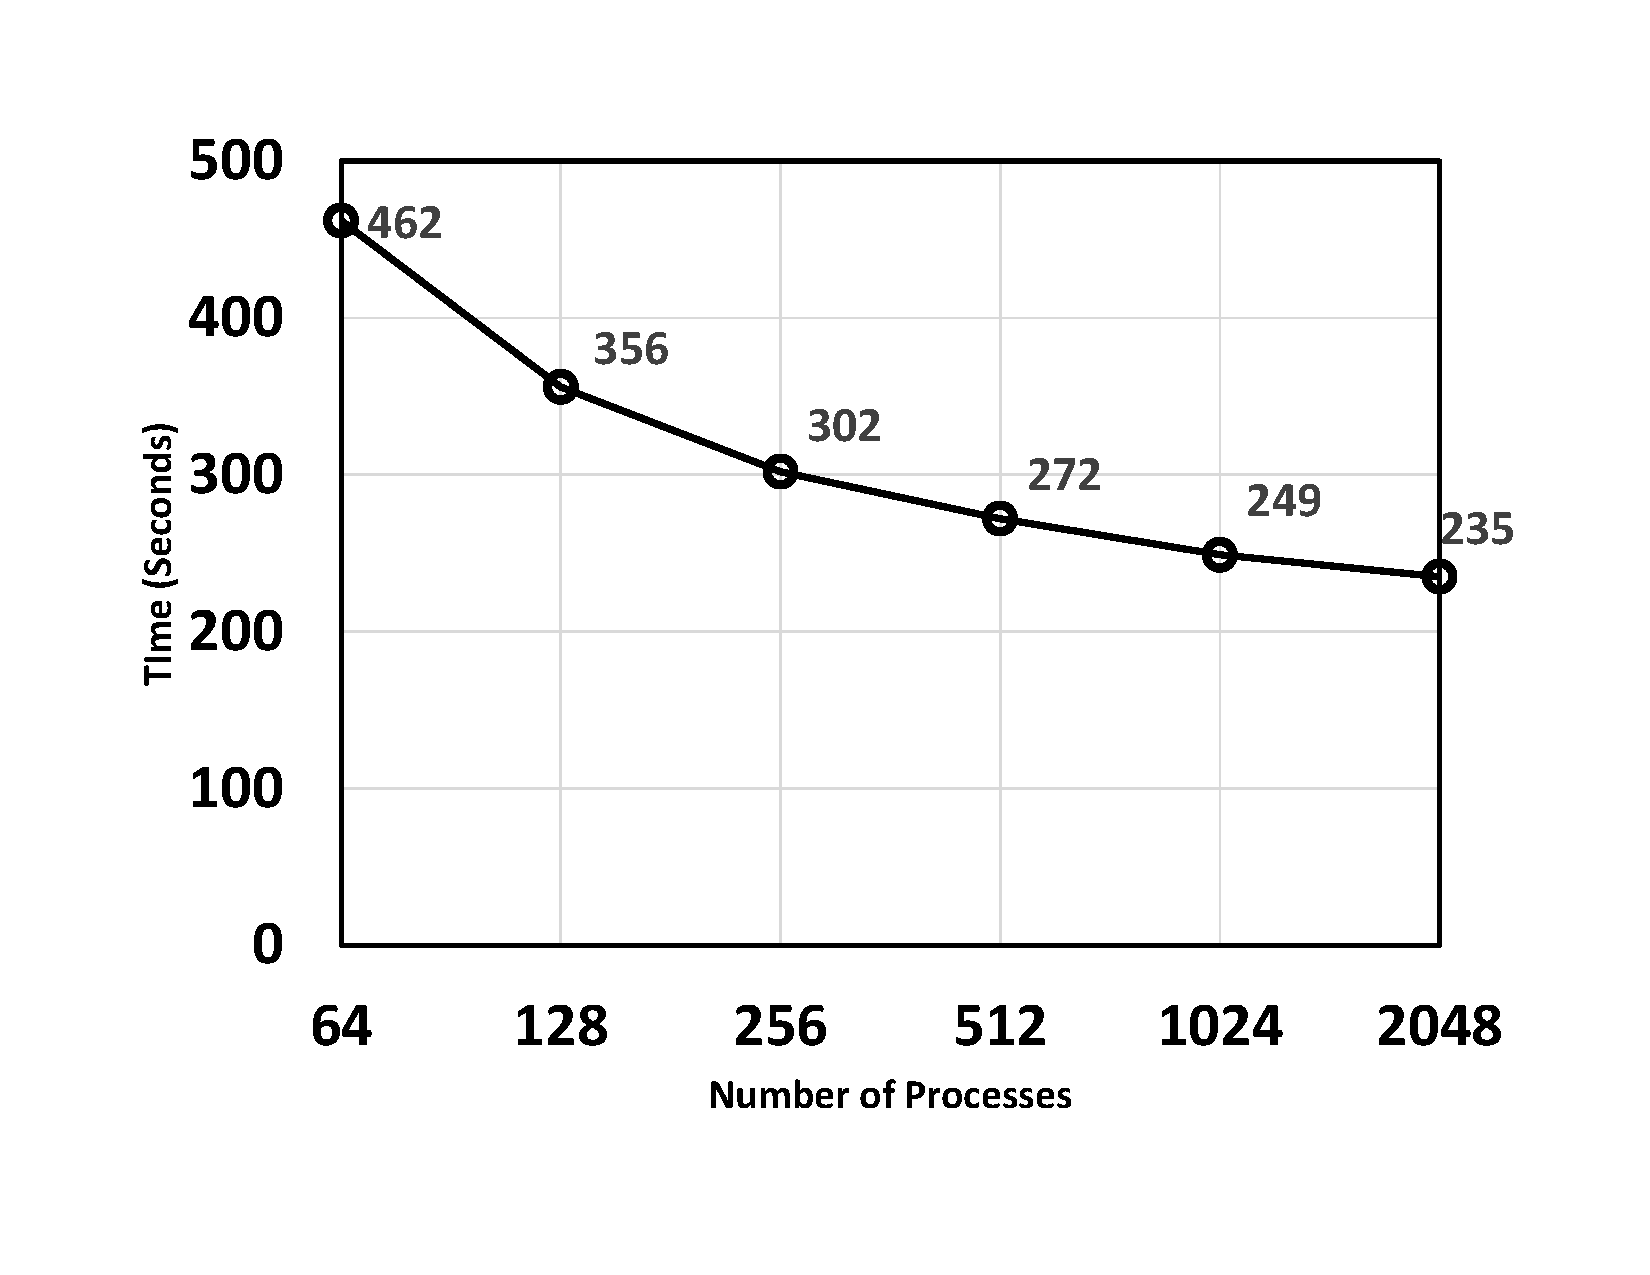
\includegraphics[trim = {25mm, 25mm, 25mm, 25mm}, width=.7\linewidth]{log/Strong_scaling.pdf}
	\caption{Strong-scaling results. \label{fig:strong_scale}}
\end{figure}
%
\begin{figure}
	\centering
	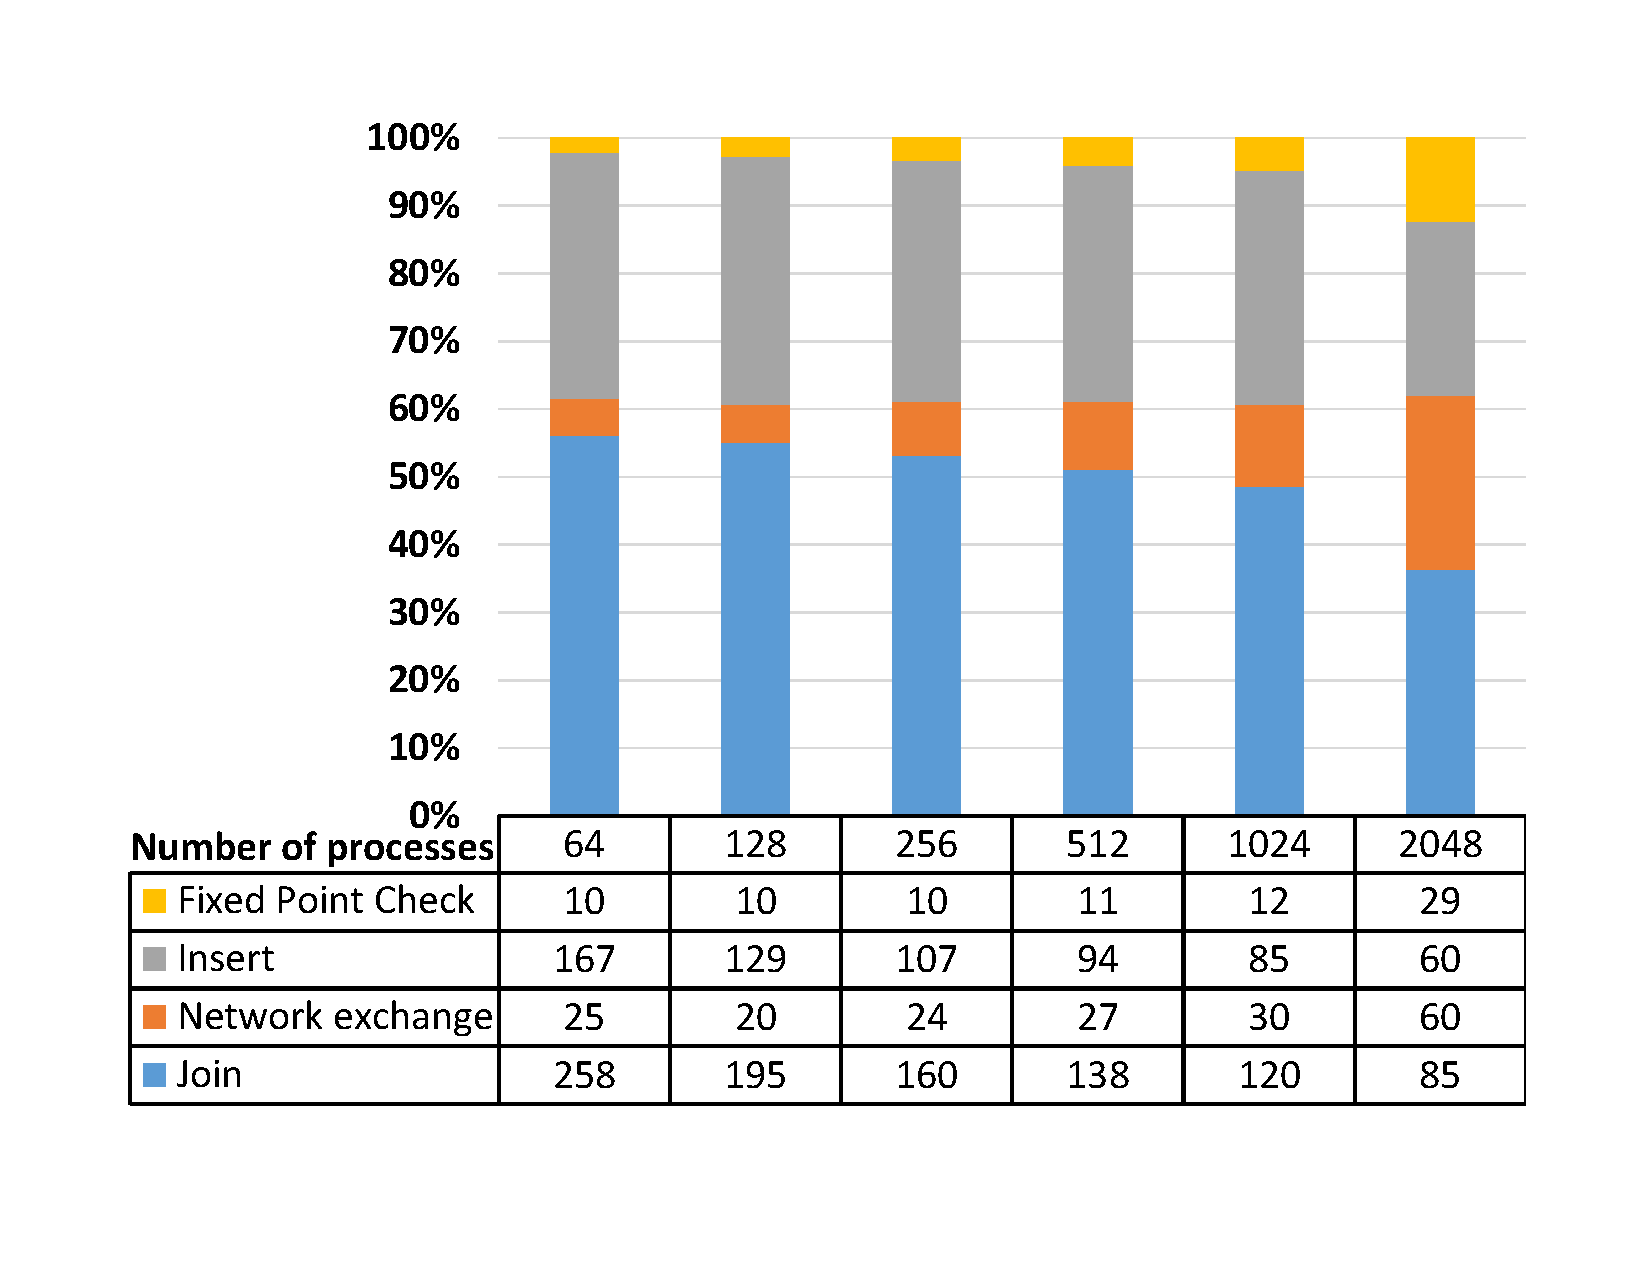
\includegraphics[trim = {25mm, 25mm, 25mm, 25mm}, width=.7\linewidth]{log/time_decomposition.pdf}
	\caption{Strong-scaling timing breakdown. \label{fig:decompose}}
\end{figure}


\subsection{Parallel Join}
%
Radix-hash join and merge-sort join are two of the most popularly used parallel implementations of the inner join operation.
Both these algorithms involve partitioning the input data so that they can be efficiently distributed 
to the participating processes. For example, in the radix-hash approach a tuple is assigned to a process 
based on the hash output of the column-value on which the join operation is keyed.
With this approach, tuples on both relations that share the same hash value
are always assigned to the same process. For every tuple in the left-hand side of the join relation is matched against all the tuples of the right-hand side of the join relation. Fast lookup data-structures like hash tables, or radix-trees (TRIE) can be used to organize the tuples within every process. The initial distribution of data using hashing reduces the overall computation overhead by a factor of the number of processes $(n)$. 

More recently ~\cite{Barthels:2017:DJA:3055540.3055545, Barthels:2015:RIJ:2723372.2750547}, there has been a concerted effort to implement JOIN operations on clusters using an MPI backend. The commonly used radix-hash join and merge-sort join have been re-designed for this purpose. 
Both these algorithms involve a hash-based partitioning of data so that they are be efficiently distributed 
to the participating processes and are designed such that inter-process communication is minimized. In both of these implementations
one-sided communication is used for transferring data between process. With one-sided communication the initiator of a data transfer request can directly access
parts of the remote memory and has full control where the data will be placed. Read and write operations are executed
without any involvement of the target machine. This approach of data transfer involves minimal synchronization between particiapting processes and have been shown to scale better that traditional two-sided communication. The implementation of parallel join has shown promising performance numbers; for example, the parallel join algorithm of~\cite{Barthels:2017:DJA:3055540.3055545}
ran successfully at 4,096 processor cores with up to 4.8 terabytes of input data.
%These results are very encouraging and we plan to extend our CFA pipeline to support MPI backend for processing datalog queries. To this end, we plan to extend the framework to work for relational operation kernels other than just the JOIN operation.


\subsection{Benchmarking: transitive closure}
%
Computing the transitive closure of a graph involves repeated join operations until a fixed point is reached.
We use the previously discussed radix-hash join algorithm to distribute the tuples across all processes.
The algorithm can then be roughly divided into four phases: 1) Join 2) network communication 3) insertion 4) checking for a fixed point.
In our join phase every process concurrently computes the join output of the local tuples. In the next phase every process sends the join output results to the relevant processes. This is a all-to-all communication phase, which we implemet using MPI's all\_to\_all routines. The next step involves inserting the join output result received from the network to the output graph's local partition. In the final step we check if the size of the output graph changed on any process, if it does then we have not yet reached a fixed point and we continue to another iteration of these 4 steps.


We performed a set of strong-scaling experiments to compute the transitive closure of graph with 412148 edges---the largest graph in the U. Florida Sparse Matrix set \cite{UF:SPMC}. We used the Quartz supercomputer at the Lawrence Livermore National Laboratory (LLNL). For our runs, we varied the number of processes from 64 to 2048. A fixed point was attained after 2933 iterations, with the resulting graph containing 1676697415 edges. As can be seen in Figure~\ref{fig:strong_scale}, our approach takes 462 seconds at 64 cores and 235 seconds at 2048 cores, corresponds to an overall efficiency of 6.25\%. We investigated these timings further by plotting the timing breakdown of by the four major components (join, network communication, join, fixed-point check) of the algorithm. We observe (see Figure~\ref{fig:decompose}) that for all our runs the total time is dominated by computation rather than communication; insert and join together tended to take up close to 90\% of the total time. This is quite an encouraging result  as it shows that we are not bound primarily by the network bandwidth (at these scales and likely moderately higher ones) and it gives us the opportunity to optimize the computation phase.




\section{Parallelizing Datalog on the GPU}
%
Programmable GPUs provide massive fine-grained parallelism, higher raw computational throughput, 
and higher memory bandwidth compared with multi-core CPUs. As a result they are a favorable  
alternative over traditional CPUs when it comes to high throughput implementations of applications.
GPU implementations can potentially provide several orders of magnitude in performance 
improvement over traditional CPUs. As a result, GPU technology is increasingly widespread
and has been successfully adopted by significant number of data-intensive
scientific applications such as molecular dynamics~\cite{ANDERSON20085342}, physical simulations~\cite{EGVE:IPT_EGVE2005:105-111},
and ray tracing in graphics~\cite{Parker:2010:OGP:1833349.1778803}.

\subsection{GPU architecture}
\begin{wrapfigure}{R}{0.45\textwidth}
	\centering
	\vspace{-0.1in}
	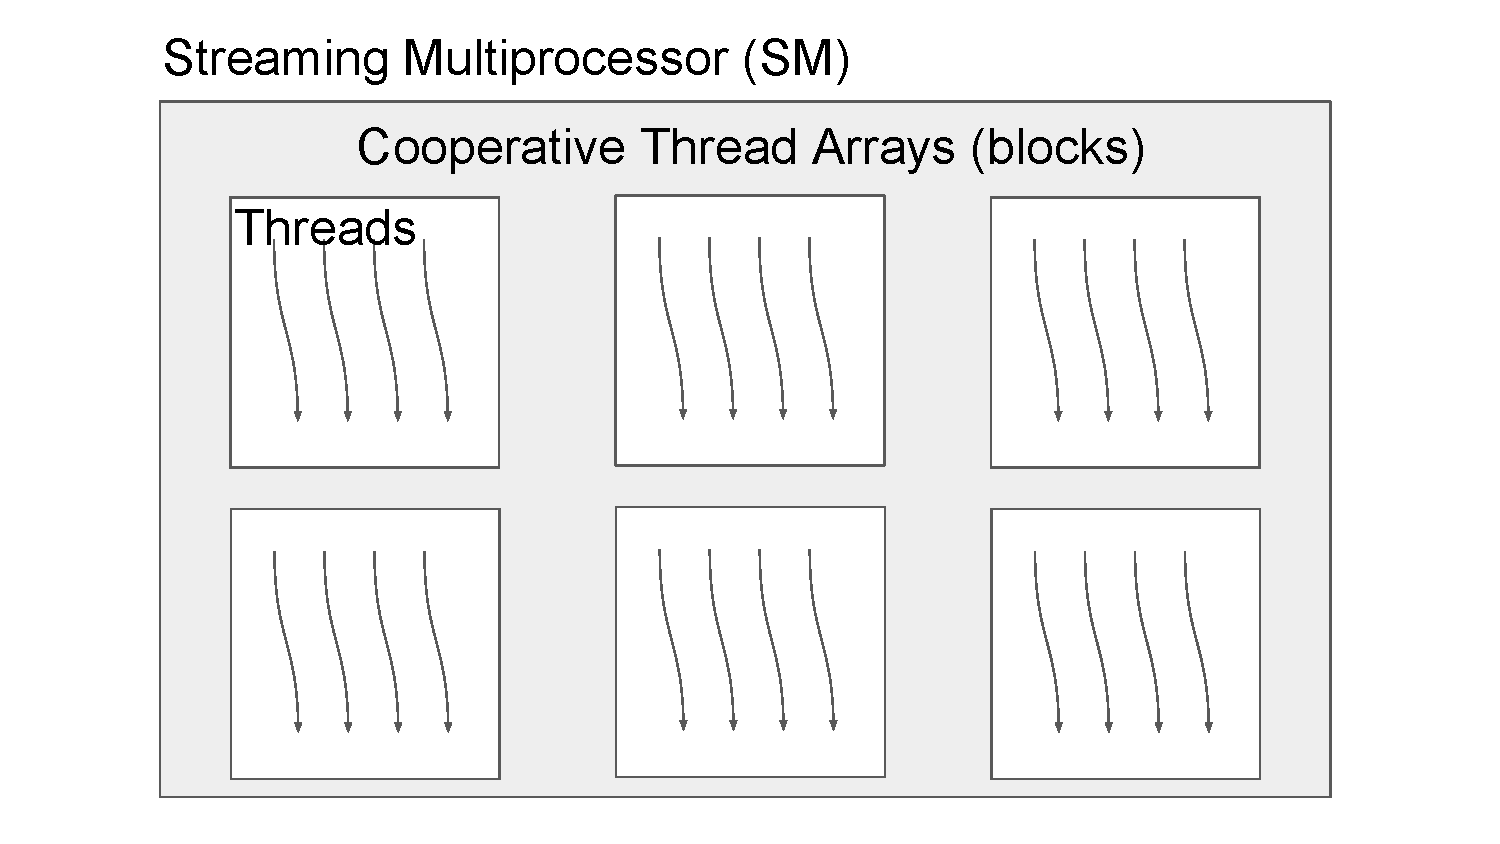
\includegraphics[width=.99\linewidth]{GPU.pdf}
	\caption{High-level overview of GPU. \label{fig:gpu}}
	\vspace{-0.2in}
\end{wrapfigure}

Threads provide the finest level of parallelism in a GPU.
A GPU application is composed of a series of multi-threaded data-parallel kernels. 
Data-parallel kernels are composed of a grid of parallel work-units called Cooperative Thread Arrays
(CTAs) which in turn consist of an array of threads. In such processors, threads within a CTA are grouped into logical units
known as warps that are mapped to SIMD units called Stream Multiprocessors (SMs) (see Figure~\ref{fig:gpu}).
The programmer divides work into threads, threads map to thread blocks (CTAs), and thread blocks map to a grid. 
The compute work distributor allocates thread blocks to SMs. 
Once a thread block is distributed to an SM the resources for the thread block are allocated 
(warps and shared memory) and threads are divided into groups of (typically) 32 threads called warps. 


\subsection{Redfox}
We use Redfox~\cite{Wu:2014:RFE:2581122.2544166} a GPU-based open-source tool to run the relational algebra (RA) kernels translated from Datalog.
Redfox is used for compiling and executing queries expressed in a specialized query language on GPUs.
Typically, the parallelism involved in solving relational-algebra operations on GPUs is challenging due to 
unstructured and irregular data access as opposed to other domain-specific operations, such as those
common to dense linear algebra. 
Redfox tackles these issues and provides an ecosystem to accelerate relational computation including
algorithm design, system implementation, and compiler optimizations. It bridges the semantic gap 
between relational queries and GPU execution models, allowing its clients to operate exclusively in terms of
RA semantics, and maintains significant performance speedup relative to the baseline CPU implementation. 

Redfox takes advantage of the fine-grained massive parallelism offered by GPUs.
It is comprised of (a) a specialized language front-end that allows the specification of sequences of RA operations
that combine to form a query, 
(b) an RA to GPU compiler, (c) an optimized GPU implementation of select RA operators, and (d) a supporting runtime.
The relational data is stored as a key-value store to support a range of workloads corresponding to queries over data
sets. We use our own system to transform datalog queries into RA kernels. Redfox provides a GPU implementation of
the following set operations:  union, intersection, difference, cross product, inner-join, project and select. Among all
the RA primitive operators,
inner-join is the most complex and is more compute intensive than the rest of the RA primitives. Another 
problem with joins is that their output size can vary, i.e. between zero to the product of the sizes of the two inputs.
One of the salient contributions of redfox is an optimal implementation of the join operation~\cite{wu_adms14}.

\subsection{Fixed-point iterations with Redfox}
\begin{wrapfigure}{R}{0.45\textwidth}
	\centering
	\vspace{-0.1in}
	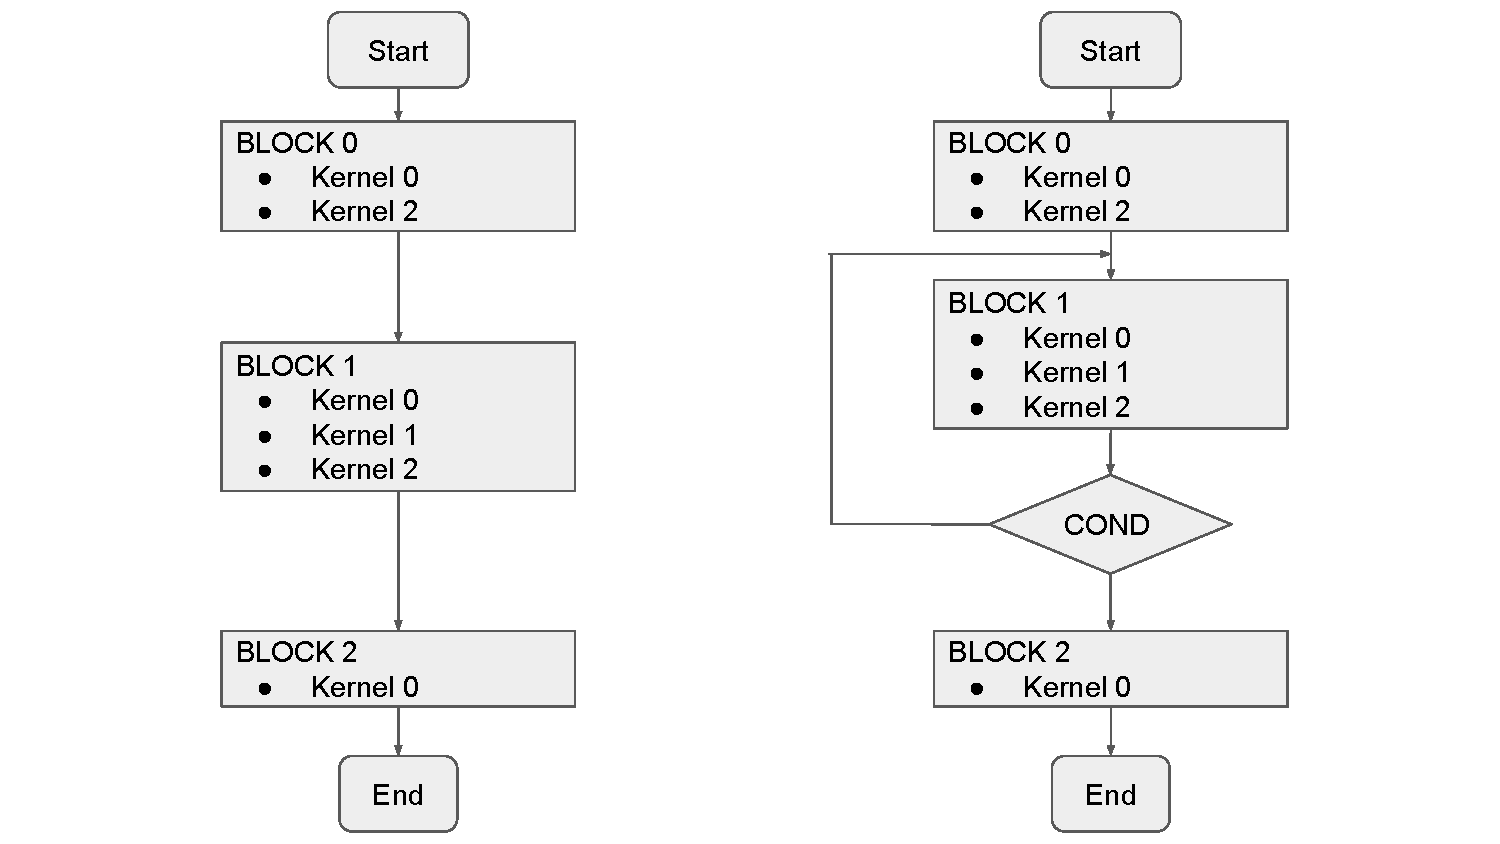
\includegraphics[width=.99\linewidth]{redfox-brances.pdf}
\caption{Redfox execution with (right) and without (left) conditional branches. \label{fig:scale}}
\vspace{-0.2in}
\end{wrapfigure}

One of the major challenges in adapting redfox to solve RA kernels derived from datalog
queries was to perform fixed-point iterations. For fixed-point iterations redfox needed to process loops and, until now, Redfox
was only used in a sequential mode, where a block unconditionally transitioned to the next block. In the original Redfox paper's experiments, the authors did use a fixed-point computation, but had manually unrolled the benchmark to the needed number of iterations. In our application,
we need the ability to run basic blocks (each a straight-line sequence of RA kernels), in a loop, until the 
relation in contention does not change and the system reaches a fixed point---regardless of how many loops this requires. 
In order to facilitate execution of loops in redfox, we have added conditional branches, that allows execution to choose a target basic block based on the equality of two input relations. We used the COND kernel of GPU and use the outcome of the kernel to schedule the target block. 
Typically, in fixed-point iterations we check if the values stored in relation after execution of a certain kernel changed or not, if it remains unchanged then
we have attained a fixed point and the execution can move forward, otherwise the set of kernel is executed again (see Figure~\ref{fig:scale}).


\subsection{Preliminary results}
%
We evaluated the performance of Redfox in computing the transitive closure of large-sized graphs. 
For benchmarking we used the open source graphs available at~\cite{UF:SPMC}.
Out of all relation operations used in computing the transitive closure, join is computationally the most complex.
We found that the join operation manage to scale decently well with larger graphs.
Time consumed performing join operation across 188 iterations
for input graph of 25,674 edges (output size is 6,489,757 edges) took 3.6 seconds. Total time for other kernel operation (project, union, copy) along with I/O time was 3.3 seconds. This total time (3.6 + 3.3 seconds) is almost comparable to the time taken by the highly optimized code Souffle (5.6 seconds) to compute the transitive closure of the same graph. We surmise, that Souffle is able to extract parallelism sufficient enough to solve the problem for this graph. Our hypothesis is that the GPU performance may become significantly faster than Souffle for very large scale graphs.







\section{Future work and Conclusion}
We have outlined a possible pipeline for extracting parallelism from a control-flow analysis in a principled way and have implemented GPU-based
and MPI-based transitive closure algorithms to experiment with parallizing this kind of problem. 
We are also interested in writing PGAS based backends for our RA kernels.
Partitioned global address space (PGAS) is a commonly used parallel programming model, 
that follows the ideals of shared memory access but operates in a distributed setting---it assumes a
global memory address space that is logically partitioned, portions of which are local to each process. 
The two main implementations of this programming model are chapel~\cite{doi:10.1177/1094342007078442} and UPC++.%~\cite{6877339}. 




\balance
\bibliographystyle{ACM-Reference-Format} 
{%\footnotesize
\bibliography{gilray,local}
}

%\iftechreport
  %\input{appendix}
%\else
%  \relax
%\fi

\end{document}

